\documentclass{suturo}
\usepackage[utf8]{inputenc}
\usepackage{listings}
\usepackage{hyperref}


\begin{document}
    \maketitle{Planning}{02.01.2017}{}{1}{}{}{}{}

\makeatletter
\newcommand{\chapterauthor}[1]{%
  {\parindent0pt\vspace*{-27pt}%
  \linespread{0}\small\begin{flushright}von: #1\end{flushright}%
  \par\nobreak\vspace*{0pt}}
  \@afterheading%
}
\makeatother


\section{Die Quellcode-Datei: main.lisp (planning\_main\_programm)}
\subsection{Architekturbild}
\chapterauthor{Kevin Störmer}


\begin{figure}[!htb]
        \center{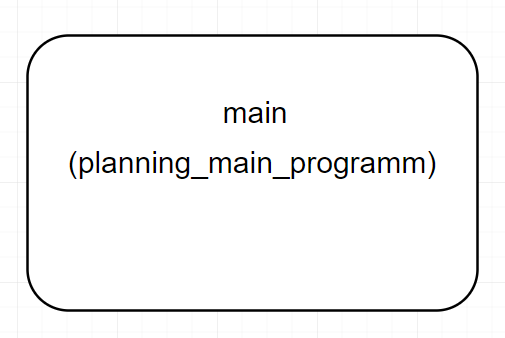
\includegraphics[width=0.4\textwidth]
        {img/diag_planning_main_programm.png}
        \caption{} Architektur der Quellcode-Datei main.lisp}
\end{figure}
      


\subsection{Beschreibung des Teilsystems}
\subsubsection{\"Ubersicht}\label{sec:main}
\chapterauthor{Kevin Störmer}
Die Die Quellcode-Datei 'main' im Paket 'planning\_main\_programm' soll ausschliesslich auf höchster Ebene den internen Ablauf des PR2 modellieren. Dabei wird der folgende Ablauf sequenziell ausgef\"uhrt:\\



\begin{figure}[!htb]
        \center{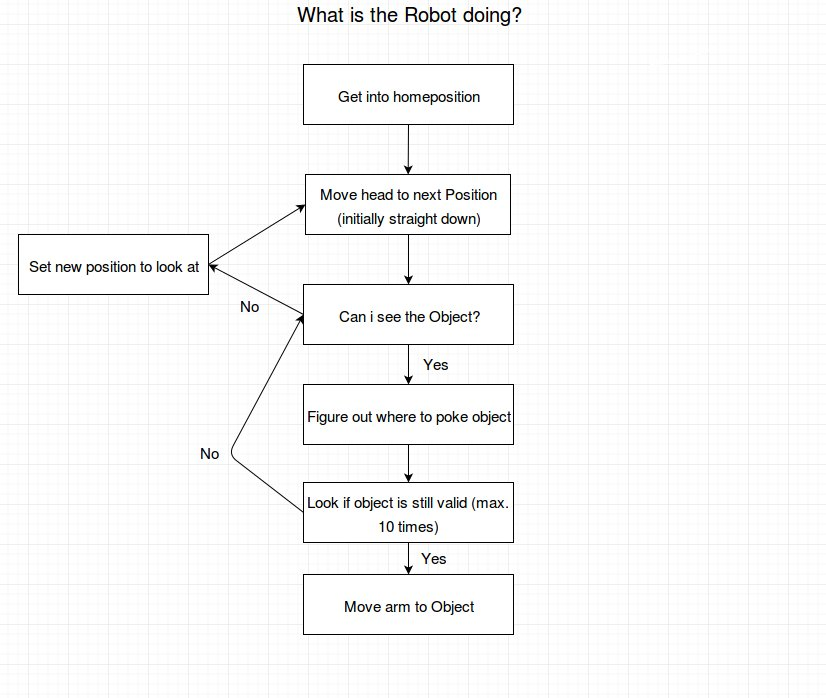
\includegraphics[width=1.0\textwidth]
        {img/diagramm.jpg}
        \caption{} Ablauf der Funktion main() }
\end{figure}


Alle dafür notwendigen Logiken, die auf Basis externer Daten entschieden werden, wurden dabei basierend auf der Quelle der Daten in andere Die Quellcode-Dateien ausgelagert. Dabei wurde z.b der Vergleich zweier Punkte aus Vision in die Die Quellcode-Datei 'points' (Paket: planning\_vision) ausgelagert.


\subsubsection{main()}
\chapterauthor{Kevin Störmer und Vanessa Hassouna}

Der Ablauf der Main wurde in \ref{sec:main} schon durch ein Schaubild dargestellt. Hier wird nun näher auf einige funktionalen Abschnitte eingegangen.



\noindent
\begin{minipage}{\linewidth}
\begin{lstlisting}
(defun main ()
  "Main function - Executing and planning robot behaviour on the top level"
  (roslisp:with-ros-node ("planning_main")
(roslisp::ros-info "Main" "Robotlife seems hard, but lets do this")
[...]
\end{lstlisting}
\end{minipage}

Die Main startet eine 'ros-nod' mit dem Namen \textit{planning\_main}. Diese node läuft solange, komplette Main einmalig durchlaufen wurde.

\noindent             
\begin{minipage}{\linewidth}
\begin{lstlisting}
[...]
(if (planning-move::find-Object 1.0 0.5)
        (progn
          (planning-motion::call-Motion-Move-Arm)
          (let ((counter 10))
            (block check-for-valid-point 
             [...]
                                                   
\end{lstlisting}
\end{minipage}             

Da die Main die Ablauf-Logik darstellt wird hier sehr oft mit dem Abfragen von Verhältnissen gearbeitet. In dem Codeabschnitt sind die Aufrufe \textbf{find-Object} sowie \textbf{call-Motion-Move-Arm} gezeigt. Die verweise auf die unteren Packete erfolgt durch \textit{Name\_des\_Packets::Name\_der\_Funktion}. \\
Darauf folgend wird eine lokale Variable \textbf{counter} erstellt die dafür zuständig ist, dass der gesamte restliche Vorgang in der Main genau 10-mal ausgeführt wird. \\
Der Block \textbf{check-for-valid-point} ist dafür da, dass innerhalb der Main gesprungen werden kann.\\

Innerhalb dieses Blocks werden alle Funktionen aufgerufen, die im nachfolgendem erklärt werden.
           
\noindent
\begin{minipage}{\linewidth}
\begin{lstlisting}
    [...]
    (return-from main  (roslisp::ros-info "Main" "Sorry i couldnt find any object :c")))))                         
    
\end{lstlisting}
\end{minipage}    

Wird kein Objekt gefunden, welches alle Anforderungen der Main erfüllt, wird die main damit unterbrochen und eine 'ros-info' ausgegeben.



\section{Die Quellcode-Datei: points.lisp (planning\_vision)}
\subsection{Architekturbild}
\chapterauthor{Kevin Störmer}



\begin{figure}[!htb]
        \center{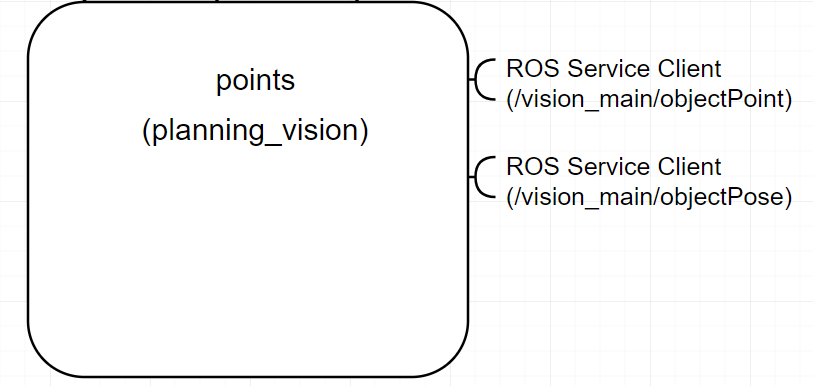
\includegraphics[width=0.6\textwidth]
        {img/diag_planning_vision.png}
        \caption{} Architektur der Quellcode-Datei points.lisp}
\end{figure}


\subsection{API}
\chapterauthor{Kevin Störmer}
\subsubsection{Serviceclients}
1. '/vision\_main/objectPoint' \\
Nimmt Objekt über Kinect wahr, und gibt Mittelpunkt des Objektes zur\"uck.\\ \\
2. '/vision\_main/objectPose' \\
Nimmt Pose (steht oder liegt) des Objektes wahr.
\subsection{Beschreibung des Teilsystems}
\subsubsection{\"Ubersicht}
\chapterauthor{Kevin Störmer}
Die Die Quellcode-Datei 'points' aus dem Paket 'planning\_vision' befasst sich ausschliesslich mit der Kommunikation mit Gruppe-Vision und Logiken auf Basis der wahrgenommenen Daten. Dabei werden Services zur Position und Pose des Objectes in Anspruch genommen und ausgewerten. Zudem wird eine Methode zur Validierung zweier Punkte angeboten.
\subsubsection{check-points-is-equal (msg-one msg-two delta)}
\chapterauthor{Kevin Störmer}

\noindent
\begin{minipage}{\linewidth}
\begin{lstlisting}
(defun check-points-is-equal (msg-one msg-two delta)
  "Compares two points with delta."
  (roslisp::ros-info "check-points-is-equal" "Starting to check if point of object is still valid")
  (roslisp:with-fields ((x1 (geometry_msgs-msg:x geometry_msgs-msg:point)) 
                        (y1 (geometry_msgs-msg:y geometry_msgs-msg:point))
                        (z1 (geometry_msgs-msg:z geometry_msgs-msg:point)))
     (object_detection-msg:position (object_detection-srv:object msg-one))
     (roslisp:with-fields ((x2 (geometry_msgs-msg:x geometry_msgs-msg:point)) 
                           (y2 (geometry_msgs-msg:y geometry_msgs-msg:point))
                           (z2 (geometry_msgs-msg:z geometry_msgs-msg:point)))
                        (object_detection-msg:position (object_detection-srv:object msg-two))
       (let (
             (dx (abs (- x1 x2)))
             (dy (abs (- y1 y2)))
             (dz (abs (- z1 z2)))
             )
         (if (and
              (<= dx delta)
              (<= dy delta)
              (<= dz delta)
              )
             (print t)
             (print nil)
             )
         )
       )
    )
  )
\end{lstlisting}
\end{minipage}

Die Funktion 'check-points-is-equal' bekommt die Parameter 'msg-one' und 'msg-two' \"ubergeben. Dabei handelt es sich um Messages vom Typ 'object\_detection-msg'. Diese enthalten Punke (x, y, z) die zu verschiedenen Zeiten von Vision über die Kinect wahrgenommen wurden. Sie stellen den Mittelpunkt des umzustossenden Objektes dar. Beim \"Ubergabeparameter delta, handelt es sich um die maximale erlaubte Tolleranz mit der die beiden Punkte von einander abweichen dürfen. \\
Anf\"anglich werden die Koordinaten der beiden Messages aus den Wrappern extrahiert und in Variablen fortan verf\"ugbar gemacht. Danach werden die Koordinaten paarweise voneinander subtrahiert um die Differenz beider als vorzeichenlose Zahl zu errechnen. Diese Differenz wird dann mit dem vorgegebenen Delta verglichen. Wenn sich alle Differenzen innerhalb des Deltas befinden, wird 'true' zurückgegeben, sonst 'nil'. 

\noindent
\begin{minipage}{\linewidth}
\subsubsection{call-vision-point ()}
\chapterauthor{Hauke Tietjen}
\begin{lstlisting}
(defvar not-a-number)

(defun call-vision-point ()
  "Call vision service, to look for point. Returns ObjectDetection object"
  (cpl:with-retry-counters ((retry-counter 10))
    (cpl:with-failure-handling
        ((cpl:simple-plan-failure (error-object)
           (format t "An error happened: ~a~%" error-object)
           (cpl:do-retry retry-counter
             (format t "Now retrying~%")
             (cpl:retry))
           (format t "Reached maximum amount of retries. Now propagating the failure up.~%")))
      (let ((response
              (roslisp:call-service
               "/vision_main/objectPoint"
               'object_detection-srv:visobjectinfo)))
        ;;Debug to find NaN message from vision
        (setf not-a-number response)
        (print not-a-number)
        (roslisp:with-fields ((x (geometry_msgs-msg:x geometry_msgs-msg:point)) 
                              (y (geometry_msgs-msg:y geometry_msgs-msg:point))
                              (z (geometry_msgs-msg:z geometry_msgs-msg:point)))
            (object_detection-msg:position (object_detection-srv:object response))
          ;;If Vision returns a NaN and it is of type String this will recover from the error
          (if (or (stringp x)
                  (stringp y)
                  (stringp z))
              (cpl:fail "One or more of the coordinates returned by the service /vision_main/objectPoint is of type String
                        which is likely the not a number error")
              (if (or (sb-ext:float-nan-p x)
                      (sb-ext:float-nan-p y)
                      (sb-ext:float-nan-p z))
                  (cpl:fail "One or more of the coordinates returned by the service /vision_main/objectPoint is  not a number")
                  (roslisp:with-fields (object_detection-msg:error) (object_detection-srv:object response)
                    (if (or (string= "Cloud empty. " object_detection-msg:error)
                            (string= "Cloud was empty after filtering. " object_detection-msg:error)
                            (string= "No plane found. " object_detection-msg:error)
                            (string= "Final extracted cluster was empty. " object_detection-msg:error))
                        (cpl:fail (concatenate 'string "Service call failed: " object_detection-msg:error))
                        (progn
                          (format t "Service call successful.")
                          (return-from call-vision-point
                            (roslisp:call-service "/vision_main/objectPoint" 'object_detection-srv:VisObjectInfo))))))))))))
\end{lstlisting}
\end{minipage}

Die Funktion 'call-vision-point' ruft den Service '/vision\_main/objectPoint' von Vision auf. Dieser Service gibt den Mittelpunkt des gesehenen Objekts zurück welcher dann nach einer Fehlerüberpüfung als 'object\_detection-msg' zurückgegeben wird. 

In Gazebo gibt dieser Service manchmal ein 'not a number' zurück, daher wird der Rückgabewert daraufhin überprüft. Es ist noch nicht klar ob 'NaN' als String oder float übergeben wird, daher wird beides überprüft. Zu 'sb-ext:float-nan-p' muss man sagen das es überprüft ob die nachfolgende Variable ein 'NaN' enthält und falls ja 't' zurückgibt, weil dazu keine Dokumentation auffindbar ist. Dann werden noch die bereitgestellten Fehlermeldungen von Vision abgefragt, z.B. ob überhaupt ein Objekt gesehen wurde. Falls mindestens eine dieser Abfragen zutrifft wird der Service-Call und die Fehlerüberprüfung neu gestartet. Dadurch kann die Funktion bis zu zehn mal neu gestartet werden bis sie endgültig aufgibt. Hier könnte in Zukunft eine Funktion auf höherem Level anknüpfen und den Kopf oder den ganzen Roboter bewegen um das Objekt doch noch zu erkennen.




\section{Die Quellcode-Datei: ask.lisp (planning\_knowledge)}
\subsection{Architekturbild}
\chapterauthor{Kevin Störmer}

\begin{center} 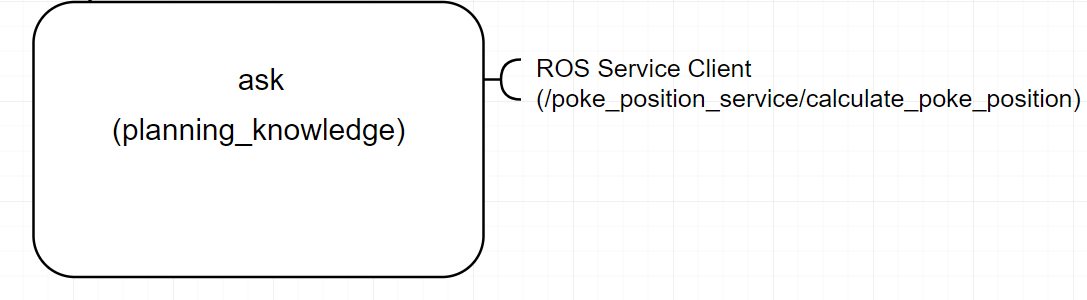
\includegraphics[width=0.8\textwidth]{img/diag_planning_knowledge.png} \end{center}



\begin{figure}[!htb]
        \center{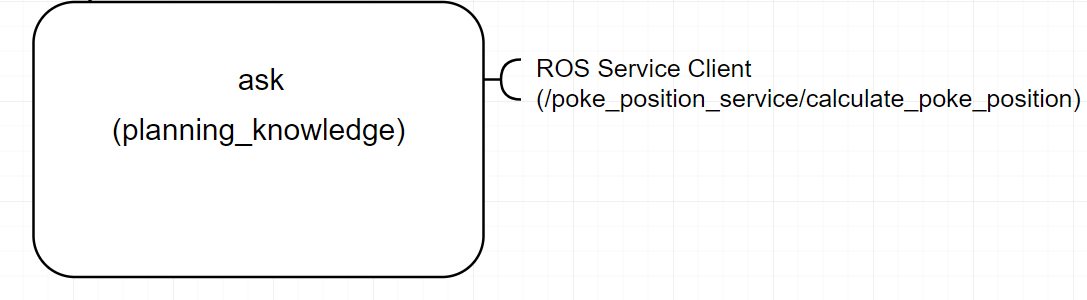
\includegraphics[width=0.8\textwidth]
        {img/diag_planning_knowledge.png}
        \caption{} Architektur der Quellcode-Datei ask.lisp}
\end{figure}


\subsection{API}
\chapterauthor{Kevin Störmer}
\subsubsection{Serviceclients}
1. '/poke\_position\_service/calculation\_poke\_position' \\
Berechnet den zu stupsenden Punkt des Objektes
\subsection{Beschreibung des Teilsystems}
\subsubsection{\"Ubersicht}
\chapterauthor{Kevin Störmer}
Die Die Quellcode-Datei 'ask' im Paket 'planning\_knowledge' ist ausschliesslich für die Kommunikation mit Gruppe Knowledge zust\"andig.
\subsubsection{ask-knowledge(point-center-of-object)}
\chapterauthor{Kevin Störmer}
Die Funktion 'ask-knowledge' bekommt als \"Ubergabeparameter eine 'object\_detection-msg' welche den, von Vision, wahrgenommenen Mittelpunkt des Objektes enthält. Knowledge gibt nach Aufruf des Services dann einen Punkt oberhalb des Mittelpunktes zur\"uck, welchen wir dann fortw\"ahrend in unserer Main weiterverwenden.

\section{Die Quellcode-Datei: actions.lisp (planning\_motion)}
\subsection{Architekturbild}
\chapterauthor{Kevin Störmer}


\begin{figure}[!htb]
        \center{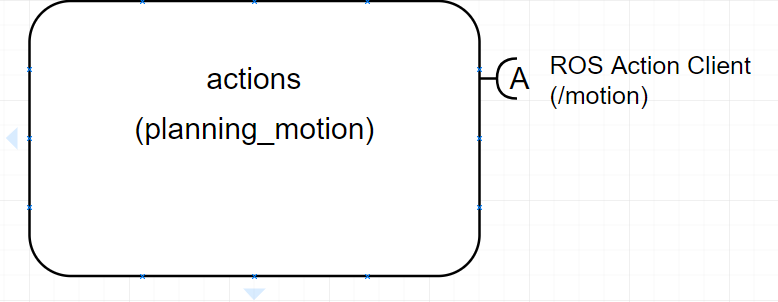
\includegraphics[width=0.6\textwidth]
        {img/diag_planning_motion.png}
        \caption{} Architektur der Quellcode-Datei actions.lisp}
\end{figure}


\subsection{API}
\chapterauthor{Kevin Störmer}
\subsubsection{Actionclients}
1. '/motion' \\
Bewegt die Arme des Pr2 entweder in die Home-Position oder zu einem bestimmten Punkt.
\subsection{Beschreibung des Teilsystems}
\subsubsection{\"Ubersicht}
\chapterauthor{Kevin Störmer}
Die Die Quellcode-Datei 'actions' im Paket 'planning\_motion'  ist ausschliesslich für die Kommunikation mit Gruppe Motion zuständig. Dabei wird die Action '/motion' einmal für die Home-Position des Pr2 und zum Bewegen des Armes zu einem bestimmten Punkt genutzt.


\subsubsection{call-Motion-Move-Arm ()}
\chapterauthor{Vanessa Hassouna}

Die Funktion call-Motion-Move-Arm im Paket 'planning\_motion' dient dazu Motion einen Befehl zu übermitteln, dass die Arme in die Standardposition (home position) gefahren werden sollen.


\noindent
\begin{minipage}{\linewidth}
\begin{lstlisting}
(defun call-Motion-Move-Arm ()
  "Moves robot-arms into home position"
  (let ((actionclient 
          (actionlib:make-action-client "/moving" "motion_msgs/MovingCommandAction")))
    (loop until
          (actionlib:wait-for-server actionclient))
    (let ((xtrans
            (cl-transforms-stamped:to-msg
             (cl-tf:make-point-stamped "base_link" 0 
                                       (cl-transforms:make-3d-vector 5.0 3.0 1.2)))))
          (let ((actiongoal 
                  (actionlib:make-action-goal actionclient point_stamped xtrans command 1)))
            (actionlib:call-goal actionclient actiongoal)))))
\end{lstlisting}
\end{minipage}

Ein \textit{actionclient} wird konstruiert auf der \textbf{action} \textit{/moving} von dem Typ \\
 \textit{motion\_msgs/MovingCommandAction}. Innerhalb der Funktion wird darauf gewartet, dass der \textit{actionclient} erstellt wird, ansonsten würde es hier zu asynchronen Abläufen kommen die zu Fehlern führen. 
Des weiteren wird aus einer konstruierten 'point-stamped' (die nur für die richtigen Übergabeparameter sorgt und keinerlei Funktionalität in diesem Beispiel hat) eine Nachricht transformiert. \\

Nun wird ein \textit{actiongoal} konstruiert, welches aus dem \textit{actionclient}, der vorherigen transformierten Nachricht und einem 'command' (von Motion definiert; 1 steht hier für die Standartposition) besteht.

\subsubsection{call-Motion-Move-To-Point (point-center-of-object)}
\chapterauthor{Vanessa Hassouna}

In dem Paket 'planning\_motion' wird die Funktion call-Motion-Move-To-Point dazu benutzt eine \textit{actiongoal} zusenden, sodass ein gewählter Arm sich zu einem Punkt bewegt.

\noindent
\begin{minipage}{\linewidth}
 
\lstset{language=PHP}
\begin{lstlisting}
[...]

    (let ((actiongoal
            (roslisp:with-fields(poke_position) point-center-of-object
              (actionlib:make-action-goal actionclient point_stamped poke_position command 3))))
[...]

\end{lstlisting}
\end{minipage}


Als Parameter wird eine Nachricht mit dem Namen \textbf{point-center-of-object} übergeben, diese kommt ursprünglich von Vision und wurde von Knowledge bearbeitet.\\
 Die Vorgehensweise ist ähnlich wie in der Funktion zuvor erklärt und wird infolgedessen hier ausgelassen.\\

 Der Unterschied der beiden Funktionen ist, dass an dieser Stelle keine Nachricht konstruiert werden muss, da diese als Parameter übergeben wird. Lediglich muss innerhalb der Nachricht auf ein Feld mit dem Namen \textbf{poke\_position} zugegriffen werden. Dieses Feld ist eine 'point\_stamped' Nachricht und wird als Wert dem \textit{actiongoal} übergeben.


\newpage
\section{Die Quellcode-Datei: movement.lisp (planning\_move)}
\subsection{Architekturbild}
\chapterauthor{Kevin Störmer}


\begin{figure}[!htb]
        \center{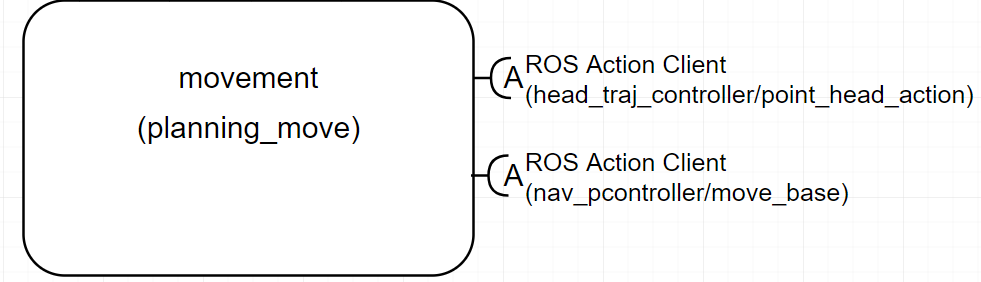
\includegraphics[width=0.8\textwidth]
        {img/diag_planning_move.png}
        \caption{} Architektur der Quellcode-Datei movement.lisp}
\end{figure}


\subsection{API}
\chapterauthor{Kevin Störmer}
\subsubsection{Actionclients}
1. 'head\_traj\_controller/point\_head\_action' \\
Bewegt den Kopf des Pr2 in Richtung eines Punktes.\\ \\
2. 'nav\_pcontroller/move\_base' \\
Bewegt die Basis des Pr2 in Richtung eines Punktes.
\subsection{Beschreibung des Teilsystems}

\subsubsection{\"Ubersicht}
\chapterauthor{Kevin Störmer}
Die Quellcode-Datei actions.lisp im Paket 'planning\_motion'  ist ausschliesslich für die Kommunikation mit Gruppe Motion zuständig. Dabei wird die Action '/motion' einmal für die Home-Position des Pr2 und zum Bewegen des Armes zu einem bestimmten Punkt genutzt.



\subsubsection{move-head (x y z)}
\chapterauthor{Kevin Störmer}

\noindent
\begin{minipage}{\linewidth}
\begin{lstlisting}
(defun move-head (x y z)
   "Moving robot head via head_traj_controller/point_head_action. X Y Z are treated as coordinates."
     (let ((actionclient 
            (actionlib:make-action-client "head_traj_controller/point_head_action" "pr2_controllers_msgs/PointHeadAction")))
       (loop until
            (actionlib:wait-for-server actionclient))
       (let ((point-to-look-at 
            (cl-transforms-stamped:to-msg 
            (cl-transforms-stamped:make-point-stamped "base_link" 0 
                                                       (cl-transforms:make-3d-vector x y z)))))
           (let ((actiongoal 
               (actionlib:make-action-goal actionclient target point-to-look-at)))
               (actionlib:call-goal actionclient actiongoal)))))
\end{lstlisting}
\end{minipage}

Die Funktion 'move-head' bekommt als \"Ubergabeparameter Koordinaten (x y z) welche vorgeben sollen, in welche Richtung der Kopf des Pr2 bewegt wird.\\
Zuerst wird ein neuer Actionclient, für die 'head\_traj\_controller/point\_head\_action' Action erstellt. Anschliessend soll in einem Loop solange gewartet werden, bis der Actionsserver gestartet wurde. Ist dies der Fall, wird eine neue Message erstellt, welche einen Punkt auf Basis der \"ubergebenen Koordinaten, in Relation zum Frame 'base\_link', enth\"alt. Diese wird dann in ein neues Actiongoal gefasst und an den Actionserver geschickt, welcher den Kopf des Pr2 dann in Richtung der Koordinaten bewegen wird.


\subsubsection{move-Base-To-Point (x y z w)}
\chapterauthor{Kevin Störmer}

\noindent
\begin{minipage}{\linewidth}
\begin{lstlisting}
(defun move-Base-To-Point (x y z w)
  "Moving robot base via nav_pcontroller/move_base. X Y Z are treated as coordinates. W for Orientation."
  (let ((actionclient 
         (actionlib:make-action-client "nav_pcontroller/move_base" "move_base_msgs/MoveBaseAction")))
     (loop until
             (actionlib:wait-for-server actionclient))
     (let ((pose-to-drive-to 
            (cl-transforms-stamped:to-msg 
            (cl-transforms-stamped:make-pose-stamped "base_link" 0 
                                                 (cl-transforms:make-3d-vector x y z) (cl-tf:make-quaternion x y z w)))))
         (let ((actiongoal 
                 (actionlib:make-action-goal actionclient target_pose pose-to-drive-to)))
                 (actionlib:call-goal actionclient actiongoal)))))
\end{lstlisting}
\end{minipage}

Die Funktion 'move-Base-To-Point' hat es nicht auf den Roboter geschafft, und ist momentan auch nicht korrekt. Sie konnte aus Zeitmangel nicht weiterentwickelt werden.\\
Angedacht war es, dass eine Pose anhand von Übergabeparametern erstellt wird, und über den Actionserver des Navp-controllers den Roboter in die vorgesehene Pose zu bewegen. Dabei traten allerdings Probleme auf, die wir zeitlich nicht mehr reparieren konnten.


\subsubsection{ask-For ()}
\chapterauthor{Vanessa Hassouna}

Die Funktion ask-For im Paket 'planning\_move' ist eine Zusatzfunktion die nur dazu dient die Nachricht von Vision auszuwerten, ob ein Objekt gefunden wurde oder nicht. Diese sollte sich in dem Packet 'planning\_vision' befinden, jedoch befindet sich diese noch in 'planning\_move'.

\noindent
\begin{minipage}{\linewidth}
\begin{lstlisting}
(defun ask-For ()
  "Asking Vision if they can see an object"
  (let ((object-Info (roslisp:call-service "/vision_main/objectPose" 'vision_msgs-srv:GetObjectInfo)))
    (roslisp:with-fields (info) object-Info (setf object-Info info))
    (roslisp:with-fields (isstanding) object-Info (setf object-Info isstanding))
    (if (= object-Info 2)
        (return-from ask-For T))))
\end{lstlisting}
\end{minipage}

Die Funktion selber braucht keinerlei Parameter. Es wird eine lokale Variable mit dem Namen \textbf{object-Info} erstellt, jene speichert die Nachricht die von Vision übermittelt wird (in dem der Service '/vision\_main/objectPose' aufgerufen wird) ab.\\

 Diese Nachricht beinhaltet zwei Felder: 1. \textit{info} und 2. \textit{isstanding}. Um an die Information im zweiten Feld zu gelangen müssen die Felder nacheinander aufgerufen werden mit \textit{roslisp:with-fields} (dieses geht auch geschachtelt). Die lokale Variable \textbf{object-Info} wird mit dem Parametern aus dem Feld \textit{isstanding} gefüllt. Dieses Feld beinhaltet die Zahl 1 oder 2, in diesem Fall steht 2 für \textbf{true} und 1 für \textbf{false}.\\
 
  Wenn also ein Objekt gefunden wurde gibt die Funktion ein true zurück, ansonsten wird automatisch ein false (nil) zurückgeliefert. 




\subsubsection{find-Object (x z)}
\chapterauthor{Vanessa Hassouna}
Die Funktion find-Object im Paket 'planning\_move' lässt den Pr2 genau \textbf{8} verschiedene Zustände durchlaufen. Dieses Vorgehen endet entweder wenn ein Objekt gefunden wurde, oder gegebenenfalls alle 8 Zustände erfolglos durchlaufen wurden.

\noindent
\begin{minipage}{\linewidth}
\begin{lstlisting}
(defun find-Object (x z)
 "Looking around from 2 to -2 to find an object"
(let ((positions (make-array '(8) 
   :initial-contents '(0.0 0.5 1 1.5 2.0 -0.5 -1.5 -2.0))))
  (loop for i across positions do
    (progn
      (let ((y i))
        (move-Head x y z))
      (if (planning-move::ask-For)
          (progn
            (roslisp::ros-info "find-Object" "I found an object, lets move on ")
            (return-from find-Object T))
          (roslisp::ros-info "find-Object" "I can't find any object, let me try it again")))))
(return-from find-Object nil))
\end{lstlisting}
\end{minipage}

 Die als Parameter übergebenen \textbf{X-} und \textbf{Z-Werte} sind festgelegt und ändern sich nicht mehr in der Funktion. Der Kopf wird hier mit der oberen Funktion move-Head bewegt. Der einzige Wert der also verändert wird ist der \textbf{Y-Wert}.\\

 Dieser führt dazu, dass der Punkt sich im Koordinatensystem (ausgehend von dem \textit{base\_link} 'frame') so verändert, dass der Pr2 nach links und rechts guckt. Die Zustände werden hier in einem Array gespeichert. Dieses Array wird durchlaufen und der jeweilige gespeicherte Wert in einer Zelle wird der Funktion move-Head (planning\_move) als \textbf{Y-Wert} übergeben (mit den Parametern die find-Object selber übermittelt bekommt).Dann wird die Funktion askFor aus dem Paket 'planning\_move' aufgerufen, jene liefert true oder false zurück wie oben beschrieben.\\
 
 Wenn also ein Objekt gefunden wurde wird eine positive Nachricht ausgegeben und ebenso eine negative für den gegenteiligen Fall.
  Wurden alle Zustände erfolglos angenommen liefert die Methode ein \textbf{false} zurück.
  
\newpage
\section{Nutzungsbeschreibung}

\subsection{Installation und Ausführung von Planning}

\subsubsection{Installation}
\chapterauthor{Vanessa Hassouna}
\begin{itemize}


\item[a] Laufen alle anderen Systeme (Vision,Knowledge und Motion) muss man für Planning folgendes Repository hinzufügen: \url{https://github.com/menanuni/planning_suturo_1718.git}. 

\item[b] Hat man erfolgreich mit \textit{catkin build} seine Arbeitsumgebung vollständig bauen können, muss man CRAM installieren \url{http://cram-system.org/installation}.

\item[c] Nun wird die Entwicklungsumgebung installiert mit: \textbf{sudo apt-get install emacs}. Achtung: Bei der Verwendung von Ubuntu 14.04 muss der neueste Lisp 'compiler' noch hinzugefügt werden \url{https://sourceforge.net/projects/sbcl/files/sbcl/1.3.1/
} (meistens x86-64 Version). Diese Datei entpacken und im Terminal (im richtigen Ordner) den Befehl: \textbf{sh install.sh} eingeben.
\end{itemize}

\subsubsection{Ausführung}
\chapterauthor{Vanessa Hassouna}
\begin{itemize}

\item Zuerst muss im Terminal \textbf{roslisp\_repl} eingeeben werden, daraufhin startet emacs. 

\item Nun wird in der Repl (dort wo cl-user steht) ein \textbf{,} (also das Komma auf der Tastertur) eingegeben.

\item Darauf folgt \textbf{r-l-s} mit \textbf{enter} und nun muss \textbf{planning\_main\_programm} mit \textbf{enter} bestätigt werden.

\item Zum Schluss wird noch in dem cl-user Fenster \textbf{(planning-main-programm::main)} eingegeben und mit \textbf{enter} bestätigt (die Klammern gehören auch dazu).
\end{itemize}


\subsection{Installation und Ausführung von Motion}

\subsubsection{Installation}
\chapterauthor{Roman Haak}
\begin{itemize}


\item[a] Zunächst müssen folgende Repositories in den source-Ordner des Workspaces hinzugefügt werden: \url{https://github.com/menanuni/motion_suturo_1718.git}, \url{https://github.com/menanuni/msgs_suturo_1718} und \url{https://github.com/menanuni/knowledge_suturo_1718.git}.

\item[b] Nun muss noch \textit{MoveIt} über den Befehl \textit{sudo apt-get install ros-indigo-moveit} und anschließend \textit{source /opt/ros/indigo/setup.bash} installiert werden.

\item[c] Jetzt kann das System über \textit{catkin build} gebaut werden.

\end{itemize}

\subsubsection{Ausführung}
\chapterauthor{Roman Haak}
\begin{itemize}

\item Zunächst muss über den Befehl \textit{roslaunch kitchen\_model\_export knowledge\_export\_service.launch} ein Teilsystem von \textit{Knowledge} gestartet werden.

\item Anschließend kann unser Knoten über \textit{roslaunch motion motion\_main\_start.launch} gestartet werden, falls er im Kontext einer Simulation ausgeführt werden soll, bzw. \textit{roslaunch motion motion\_main\_start\_real\_pr2.launch}, falls der Knoten auf dem PR2 ausgeführt werden soll.

\item Dann können Befehle an den Actionserver unseres Knotens über das Topic \textit{/moving/goal} abgesetzt werden. Zur Erläuterung des Actionservers siehe Dokumentation der Gruppe \textit{motion}.
\end{itemize}


\subsection{Installation und Ausführung von Vision}

\subsubsection{Installation}
\chapterauthor{Alexander Link}

\textbf{Voraussetzungen}

\begin{itemize}
\item Ubuntu 14.04
\item ROS Indigo
\item Catkin tools
\item Gazebo 2.2.x
\end{itemize}

\textbf{.bashrc}

Folgendes muss zur .bashrc (oder zshrc) hinzugefügt werden:
\begin{itemize}
\item \textit{export KINECT1=true}
\item \textit{export GAZEBO\_MODEL\_PATH= \$HOME/catkin\_ws/vision\_suturo\_1718/vision/models}
\item \textit{export GAZEBO\_RESOURCE\_PATH= \$HOME/catkin\_ws/vision\_suturo\_1718/vision/worlds}
\end{itemize}

\textbf{Setup}

\begin{itemize}
\item gazebo installieren: \textit{sudo apt-get install ros-indigo-pr2-simulator}

\item Sollten Probleme auftreten, könnte dies durch ein Update von gazebo auf v2.2.6 gelöst werden:
\\
\textit{sudo sh -c 'echo "deb http://packages.osrfoundation.org/gazebo/ubuntu trusty main" > /etc/apt/sources.list.d/gazebo-latest.list'}
\\
\textit{wget http://packages.osrfoundation.org/gazebo.key -O - | sudo apt-key add -}
\\
\textit{sudo apt-get update}

\item Folgende Pakete in den src-Ordner eines catkin workspaces klonen:\\
        \textbf{vision\_suturo\_1718} (this package) \\
        \textbf{msgs\_suturo\_1718}
\item Erst "\textit{catkin build object\_detection}" nutzen, um die messages zu bauen.
\item Dann "\textit{catkin build}" benutzen, um alles andere zu bauen.

\end{itemize}

\textbf{Kinect benutzen}
\begin{itemize}
\item \textit{sudo apt install ros-indigo-freenect-launch freenect libfreenect-bin}
\item \textit{roslaunch freenect\_launch freenect-registered-xyzrgb.launch}
\item (Optional) \textit{roslaunch vision vision\_kinect.launch}
\end{itemize}

\textbf{Dateien speichern}

    \textit{rosrun pcl\_ros pointcloud\_to\_pcd input:=/camera/depth\_registered/point}


\subsubsection{Ausf\"uhrung}
\chapterauthor{Alexander Link}

\textbf{vision\_main/objectPoint}
\begin{itemize}
\item Liefer einen PointStamped und einen Fehlercode zurück
\item Nimmt keine Argumente
\item Benutzt VisObjectInfo.srv
\end{itemize}
\textbf{vision\_main/objectPose (WIP)}
\begin{itemize}
\item Gibt einen bool zur\"uck, der angibt, ob ein Objekt steht oder liegt, zusammen mit einem String f\"ur weitere Informationen.
\item Nimmt keine Argumente
\item Benutzt GetObjectInfo.srv 
\end{itemize}

\textbf{rosservice}

Unsere Services k\"onnen auch manuell abgerufen werden: \\

\textit{rosservice call vision\_main/objectPoint} \\

oder \\

\textit{rosservice call vision\_main/objectPose}

\subsection{Installation und Ausführung von Knowledge}

\subsubsection{Installation}
\chapterauthor{Alexander Haar}

\begin{itemize}
\item[1.] Java8 installieren: \href{https://wiki.ubuntuusers.de/Java/Installation/Oracle_Java/Java_8/}{klick mich} Wichtig JDK
\item[2.] Repo clonen und bauen
\item[3.] Die folgenden Schritte ausführen: \href{http://knowrob.org/installation/workspace}{klick mich}
\end{itemize}

\subsubsection{Ausführung}
\chapterauthor{Alexander Haar}

Um alle wichtigen Knoten zu starten muss einfach der Befehl \textit{roslaunch knowledge knowledge\_main.launch} ausgeführt werden. Es wird eine json\_prolog- Node, der PokePositon-Service und der GetFixedKitchenModel- Service gestartet.
\end{document}

